\subsection{Experiment 4: Characteristics of Metrics in Regression Tasks}

\begin{figure}[H]
    \centering
    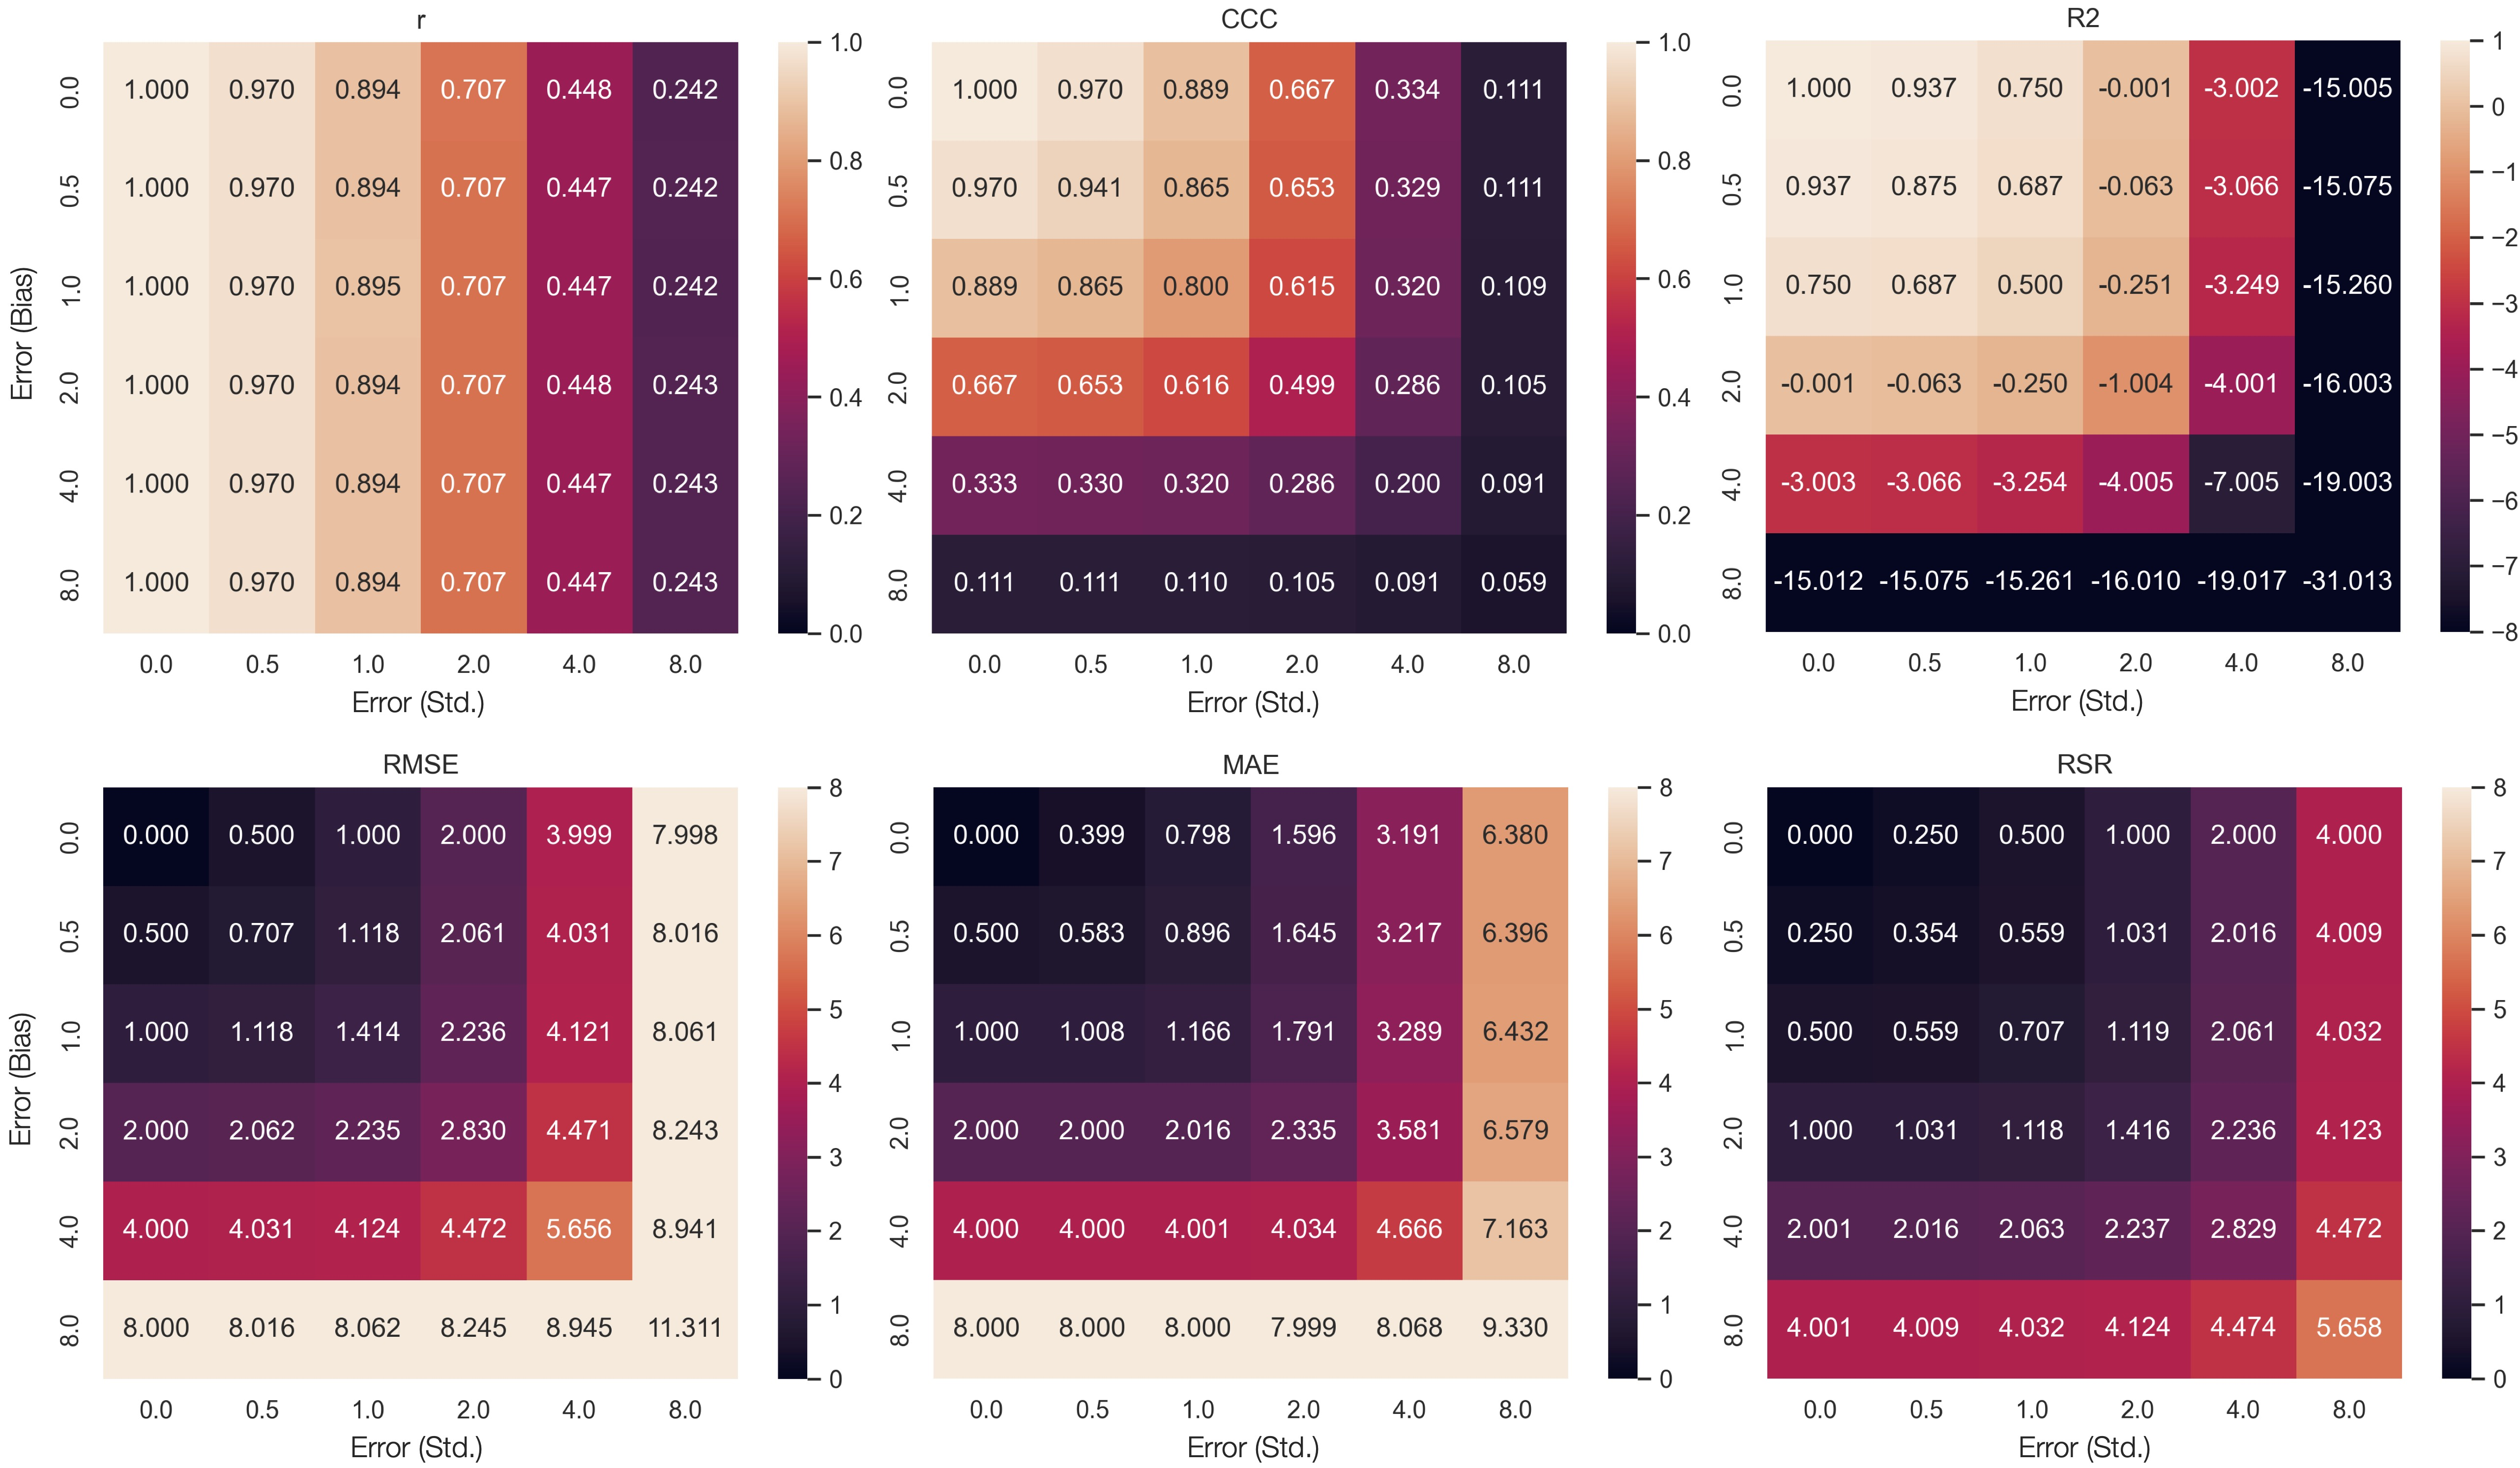
\includegraphics[width=1\textwidth]{fig_9.jpg}
    \caption{Heatmaps illustrating various metrics as functions of the bias and standard deviation (Std.) of the prediction error in a regression task, where the ground truth values have a Std. of 4.}
    \label{fig:s4_reg}
\end{figure}

Metrics in regression tasks exhibit distinct trends in response to various combinations of error bias and variance (Figure \ref{fig:s4_reg}). Except for $r$ and MAE, all metrics demonstrate symmetric responses in the grid matrix, supporting the trade-off relationship between bias and variance. For instance, $R^2$ consistently shows a value of 0.75 at the positions (1, 4) and (4, 1), indicating that a model with zero bias and variance of 2 achieves the same $R^2$ as a model with bias of 2 and zero variance.

Both $r$ and CCC are linearity-based metrics that assess the correlation between predicted and actual values, yet they exhibit different trends in the heatmap. Since $r$ is standardized by the standard deviation of both predicted and actual values, it is entirely invariant to bias errors, which reflect the scale of the prediction error. In contrast, CCC is sensitive to both bias and variance, offering a more comprehensive evaluation of correlation. In this experiment, CCC also provides better interpretability compared to $r$. Specifically, when \text{CCC} > 0.5, the total squared error (i.e., the sum of squared bias and variance) does not exceed $4 + 4 = 8$, which is twice the ground truth variance ($2^2 = 4$). Furthermore, when \text{CCC} > 0.8, the error is guaranteed to be less than the ground truth variance. Unlike the ambiguous interpretation of r, these benchmarks provide a straightforward guideline for translating the correlation concept into the scale of prediction errors.

$R^2$ is a widely used metric in the machine learning community and offers good interpretability. When $R^2 = 0$, it indicates that the model performs no better than the mean prediction. In the heatmap, this is evident at positions (4, 1) and (1, 4), where the prediction error equals the ground truth variance. Additionally, when $R^2 = -1$, it suggests the prediction error exceeds the mean prediction error by one unit of the ground truth variance, as seen at position (4, 4), where both bias and variance errors are 2, resulting in a total squared error of 8 (twice the ground truth variance). Although $R^2$ shares similar interpretability with CCC, it inflates rapidly in the presence of outliers. For example, when the bias or variance error increases from 4 to 8, $R^2$ drops dramatically from -3 to -15. In contrast, CCC decreases only by 0.22 under the same conditions, maintaining a range between 0 and 1, which makes it more stable and comparable across different prediction contexts.

Error-based metrics like RMSE and MAE are often compared for their robustness to outliers. Due to the squared error term in RMSE, it is more sensitive to large prediction errors. Interestingly, when analyzing their response to increases in bias error, RMSE and MAE exhibit identical trends: a 1-unit increase in bias error results in a 1-unit increase in both metrics. However, differences emerge along the variance error axis, where MAE increases by only 0.8 units per unit increase in variance error, whereas RMSE increases by 1 unit. This indicates that MAE is more robust to variance-related errors than RMSE, making it better suited for handling outlier predictions.

RSR, on the other hand, standardizes RMSE by the standard deviation of the ground truth values. In this experiment, where the ground truth values were generated from a normal distribution with a standard deviation of 2, RSR serves as a direct comparison to RMSE. While RMSE reflects the original error scale, RSR normalizes the error scale to the ground truth variance, resulting in values that are always half those of RMSE. This property makes RSR an excellent metric for comparing model performance across multiple datasets with varying variance levels. RSR provides a uniform standard for performance evaluation while retaining the capability to capture error amplitude, which linearity-based metrics like $r$ and CCC lack.
